\chapter{Entropi dan Energi Bebas Reaksi}\label{ch:b2:reaction-free-energy}

Kompres dingin untuk olahraga berisi sebuah kantong air dan beberapa
sendok amonium nitrat. Jika kompres itu ditekan, kantong di dalamnya
pecah, garamnya larut, dan dalam beberapa detik kompres itu cukup dingin
untuk meredakan pergelangan kaki yang terkilir. Pelarutan itu menyerap
kalor --- prosesnya \omterm{def:b2:reaction-enthalpy:exothermic}{endoterm} --- tetapi tetap berlangsung dengan
sendirinya, sampai tuntas. Entalpi pada bab sebelumnya tidak mungkin
menjadi keseluruhan cerita: reaksi tidak hanya berjalan ``menuruni bukit
kalor''. Besaran yang hilang adalah entropi, yang oleh hukum kedua
termodinamika, yang sudah dijumpai dalam fisika, dijadikan hakim bagi
setiap perubahan spontan. Bab ini menabelkan entropi, menghitung \omterm{def:b2:reaction-free-energy:reaction-entropy}{entropi
reaksi}, dan menggabungkan entalpi dan entropi menjadi satu fungsi, yaitu
\omterm{def:b2:reaction-free-energy:gibbs-energy}{energi Gibbs}, yang turunannya terhadap reaksi menentukan arah setiap
reaksi pada suhu dan tekanan tetap.

\begin{recall}
Dari fisika: hukum kedua. Setiap sistem mempunyai sebuah fungsi keadaan,
yaitu entropinya $S$ (ekstensif); dalam transformasi sistem tertutup,
$\dd S =
\delta Q/T_{\text{ext}} + \delta S_{\text{c}}$, dengan entropi
tercipta $\delta S_{\text{c}}$ bernilai nol untuk perubahan reversibel dan
positif untuk perubahan lainnya; untuk sistem tertutup dengan komposisi
tetap, $\dd U = T\dd S -
p\dd V$. \Cref{ch:b2:reaction-enthalpy}: \omterm{def:b2:reaction-enthalpy:reaction-quantity}{besaran
reaksi} $\Delta_r X =
(\partial X/\partial\xi)_{T,p}$ dan \omterm{def:b2:reaction-enthalpy:standard-reaction-enthalpy}{entalpi reaksi
standar}. Jilid Tahun 1 menyatakan, sebagai hukum ``yang diturunkan dari
hukum kedua'', bahwa sebuah reaksi berevolusi sampai $Q = K^\circ$; bab
ini dan dua bab berikutnya menurunkannya.
\end{recall}

\begin{omfigure}
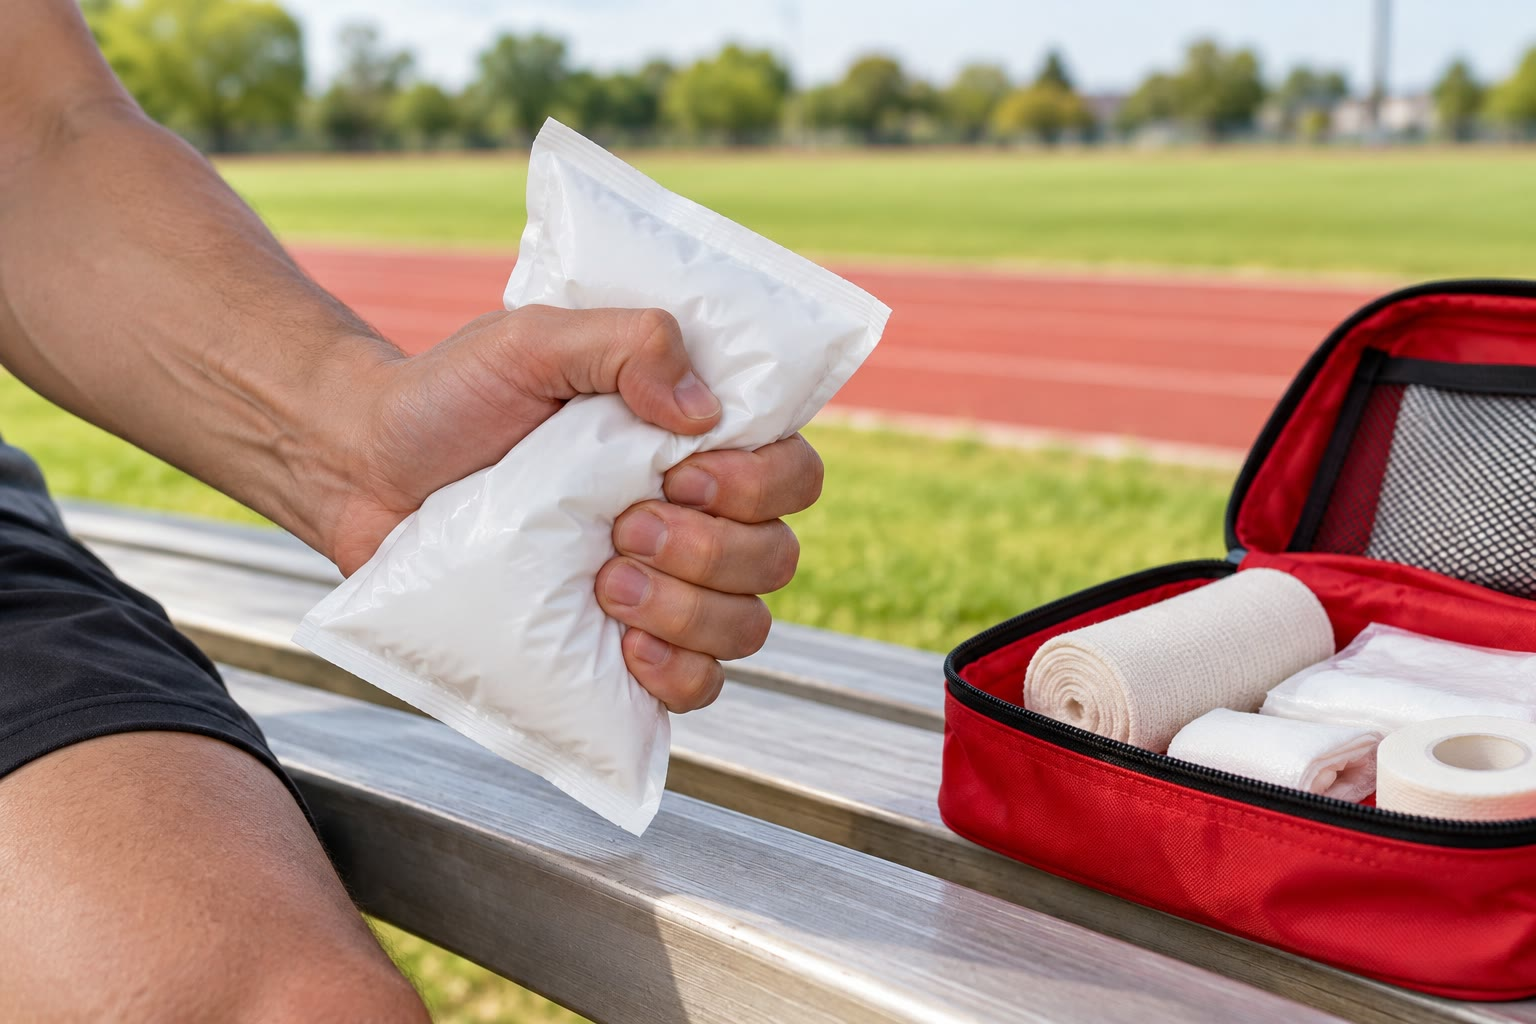
\includegraphics[width=0.55\linewidth]{images/book3/ai/b2-02-cold-pack.jpg}

{\small Kompres dingin: ketika kantong di dalamnya dipecahkan, amonium
nitrat larut dalam air dan kompres itu menjadi dingin. Pelarutan itu
\omterm{def:b2:reaction-enthalpy:exothermic}{endoterm} dan spontan; entropinya menjelaskan mengapa
(\cref{ex:b2:reaction-free-energy:cold-pack}).}
\end{omfigure}

\section{Entropi standar dan hukum ketiga}

Berbeda dengan entalpi, entropi mempunyai titik nol alami.

\begin{theorem}[Hukum ketiga termodinamika]\label{thm:b2:reaction-free-energy:third-law}
Entropi sebuah kristal murni yang tersusun sempurna menuju nol ketika
suhunya menuju \qty{0}{K}.
\end{theorem}
\admitted

\begin{remark}[Dari mana titik nol itu berasal]\label{rem:b2:reaction-free-energy:third-law}
Walther Nernst menyatakan pada tahun 1906 bahwa \omterm{def:b2:reaction-free-energy:reaction-entropy}{entropi reaksi} antara
fase-fase terkondensasi lenyap ketika $T \to 0$; Max Planck mempertajamnya
menjadi pernyataan di atas. Asal-usulnya bersifat statistik: entropi
menghitung susunan mikroskopis yang sesuai dengan keadaan sebuah sistem,
dan kristal sempurna pada \qty{0}{K} hanya mempunyai satu susunan.
Perhitungan itu dilakukan dalam jilid Tahun 3, dengan fungsi partisi.
\end{remark}

\begin{definition}[Entropi molar standar]\label{def:b2:reaction-free-energy:standard-entropy}
Yang disebut \emph{entropi molar standar}\index{entropi molar standar}
$S^\circ_m(T)$ sebuah zat adalah entropi satu mol zat itu dalam keadaan
standarnya pada suhu $T$, dengan titik nol menurut hukum ketiga. Berbeda
dengan $\Delta_f H^\circ$, entropi ini merupakan besaran mutlak, yang
bernilai positif untuk setiap zat, termasuk unsur-unsur.
\end{definition}

\begin{proposition}[Entropi mutlak dari kapasitas kalor]\label{prop:b2:reaction-free-energy:absolute-entropy}
Dengan memanaskan sebuah zat pada tekanan tetap $p^\circ$ dari \qty{0}{K} sampai $T$,
\[
  S^\circ_m(T) = \int_0^T\frac{C^\circ_{p,m}(T')}{T'}\,\dd T' +
  \sum_{\text{transisi}}\frac{\Delta_{\text{trs}}H^\circ}{T_{\text{trs}}} ,
\]
dengan integral yang diambil dalam setiap fase pada rentang suhunya.
\end{proposition}

\begin{proof}
Panaskan zat itu secara reversibel pada tekanan tetap: $\delta S_{\text{c}} =
0$ dan $\delta Q = \dd H = C_p\,\dd T$, sehingga $\dd S = C_p\,\dd T/T$. Pada
suatu transisi (peleburan, pendidihan), suhu tetap pada $T_{\text{trs}}$
sementara kalor $\Delta_{\text{trs}}H$ diterima secara reversibel: entropi
melonjak sebesar $\Delta_{\text{trs}}H/T_{\text{trs}}$. Jumlahkan
bagian-bagian itu mulai dari titik nol hukum ketiga.
\end{proof}

\begin{omfigure}
\begin{tikzpicture}
\begin{axis}[
  width=0.8\linewidth, height=6.2cm, xmin=0, xmax=1500, ymin=0, ymax=210,
  axis x line=bottom, axis y line=left, xlabel={$T$ (K)},
  ylabel={$S^\circ_m$ seng (\unit{J/(K.mol)})},
  xtick={0,250,500,750,1000,1250,1500},
  tick label style={font=\small}, label style={font=\small}, clip=false]
\addplot[omDef, very thick, smooth] table[x=T, y=S] {figdata/out/bachelor-2-standard-entropy-solid.dat};
\addplot[omProp, very thick] table[x=T, y=S] {figdata/out/bachelor-2-standard-entropy-liquid.dat};
\addplot[omThm, very thick] table[x=T, y=S] {figdata/out/bachelor-2-standard-entropy-gas.dat};
\draw[densely dashed, gray] (axis cs:692.73,64.6) -- (axis cs:692.73,75.2);
\draw[densely dashed, gray] (axis cs:1180.2,91.9) -- (axis cs:1180.2,189.6);
\node[omDef, font=\small, anchor=south east] at (axis cs:600,60) {padat};
\node[omProp, font=\small, anchor=north west] at (axis cs:850,78) {cair};
\node[omThm, font=\small, anchor=south] at (axis cs:1350,192) {gas};
\node[font=\scriptsize, anchor=west, align=left] at (axis cs:700,110) {peleburan, $+10.6$\\ pada \qty{692.7}{K}};
\node[font=\scriptsize, anchor=east, align=right] at (axis cs:1170,150) {pendidihan,\\ $+97.7$ pada\\ \qty{1180.2}{K}};
\end{axis}
\end{tikzpicture}

{\small \omterm{def:b2:reaction-free-energy:standard-entropy}{Entropi molar standar} seng dihitung dari titik nol hukum ketiga.
Entropi itu bertambah seiring suhu karena logam menyimpan kalor, lalu
melonjak pada titik lebur sebesar $\Delta_{\text{fus}}H/T_{\text{fus}}$
dan, jauh lebih besar, pada titik didih sebesar
$\Delta_{\text{vap}}H/T_b$: gas jauh lebih tidak teratur daripada
cairan.}
% ledger: s0T:Zn_crl.0, s0T:Zn_crl.298.15, s0T:Zn_cr.692, s0T:Zn_l.692, s0T:Zn_l.1180, s0T:Zn_g.1180, hT:Zn_cr.692, hT:Zn_l.692, hT:Zn_l.1180, hT:Zn_g.1180, dfh:Zn_g (curve in figdata/bachelor-2/standard-entropy.py)
\end{omfigure}

Gambar ini memberikan orde besaran yang patut diingat. Pada suhu kamar,
logam atau kristal keras mempunyai entropi beberapa puluh
\unit{J/(K.mol)}, cairan sekitar seratus, gas seratus hingga tiga ratus;
peleburan menambahkan sedikit, pendidihan menambahkan banyak. \omterm{def:b2:reaction-free-energy:standard-entropy}{Entropi
molar standar} yang dipakai dalam jilid ini ditabelkan bersama entalpi
pembentukan.

\section{Entropi reaksi}

\begin{definition}[Entropi reaksi]\label{def:b2:reaction-free-energy:reaction-entropy}
Yang disebut \emph{entropi reaksi}\index{entropi reaksi} adalah
$\Delta_r S =
(\partial S/\partial\xi)_{T,p}$, dan \emph{entropi reaksi
standar}\index{entropi reaksi standar} adalah $\Delta_r S^\circ(T) =
\sum_i\nu_iS^\circ_{m,i}(T)$, dalam \unit{J/(K.mol)}.
\end{definition}

Karena entropi standar bersifat mutlak, tidak diperlukan reaksi
pembentukan: unsur-unsur diperhitungkan dengan entropinya sendiri.

\begin{example}[Tiga entropi reaksi]\label{ex:b2:reaction-free-energy:entropies}
Pada \qty{298.15}{K}:
\begin{itemize}
  \item \ce{CaCO3(s) -> CaO(s) + CO2(g)}: $\Delta_r S^\circ = 39.75 + 213.79 -
        92.9 = \qty{+160.6}{J/(K.mol)}$, gas yang dibuat dari padatan;
  \item \ce{N2(g) + 3H2(g) -> 2NH3(g)}: $\Delta_r S^\circ = 2(192.77) -
        191.61 - 3(130.68) = \qty{-198.1}{J/(K.mol)}$, empat molekul gas
        menjadi dua;
  \item \ce{N2O4(g) -> 2NO2(g)}: $\Delta_r S^\circ = 2(240.03) - 304.38 =
        \qty{+175.7}{J/(K.mol)}$.
\end{itemize}
% ledger: s0:CaCO3_cr, s0:CaO_cr, s0:CO2_g, s0:N2_g, s0:H2_g, s0:NH3_g, s0:N2O4_g, s0:NO2_g (computed in figdata/bachelor-2/thermo-data.py)
\end{example}

\begin{proposition}[Tanda entropi reaksi]\label{prop:b2:reaction-free-energy:sign-rule}
Jika gas ikut bereaksi, tanda $\Delta_r S^\circ$ pada umumnya sama dengan
tanda $\Delta\nu_{\text{gas}} = \sum_{\text{gas}}\nu_i$, dan besarnya
sekitar \qty{100}{} sampai \qty{200}{J/(K.mol)} per mol gas yang dibentuk
atau dikonsumsi. Jika $\Delta\nu_{\text{gas}} = 0$, atau tidak ada gas
yang terlibat, $\Delta_r S^\circ$ kecil dan tandanya harus dihitung.
\end{proposition}

\begin{proof}[Pembenaran]
Entropi molar gas pada \qty{298}{K} berada di antara 130 dan
\qty{300}{J/(K.mol)}, sedangkan entropi molar padatan atau cairan beberapa
puluh: pembentukan atau konsumsi satu mol gas mendominasi semua
sumbangan lainnya. Ini adalah aturan praktis, bukan teorema: pelarutan
sebuah garam, tanpa gas, tetap dapat mengubah entropi sebesar seratus
\unit{J/(K.mol)}.
\end{proof}

\begin{method}[Meramalkan tanda $\Delta_r S^\circ$]\label{met:b2:reaction-free-energy:entropy-sign}
\begin{enumerate}
  \item Hitunglah $\Delta\nu_{\text{gas}}$: jika tidak nol, nilai itulah
        yang memberikan tandanya.
  \item Jika nol, bandingkan keteraturan keadaan-keadaannya: melarutkan
        kristal, melebur, memecah sebuah molekul menjadi dua bagian
        menaikkan entropi; mengendapkan, membeku, menggabungkan dua molekul
        menjadi satu menurunkannya.
  \item Jika keputusannya penting, hitunglah $\sum_i\nu_iS^\circ_{m,i}$.
\end{enumerate}
\end{method}

Jilid Tahun 1 telah menjumpai salah satu akibatnya: eliminasi
menghasilkan lebih banyak molekul daripada substitusi dengan pereaksi
yang sama (alkena, gugus pergi, dan basa terprotonasi, dibandingkan dengan
produk substitusi dan gugus pergi). \omterm{def:b2:reaction-free-energy:reaction-entropy}{Entropi reaksinya} lebih besar, dan
suku entropi, yang bertambah seiring suhu seperti ditunjukkan pada subbab
berikutnya, itulah sebabnya pemanasan lebih menguntungkan eliminasi
daripada substitusi.

\section{Energi Gibbs}

\begin{definition}[Energi Gibbs]\label{def:b2:reaction-free-energy:gibbs-energy}
Yang disebut \emph{energi Gibbs}\index{energi Gibbs} (atau entalpi bebas)
sebuah sistem adalah fungsi keadaan $G = H - TS$, yang ekstensif, dalam
joule.
\end{definition}

\begin{definition}[Energi Gibbs reaksi]\label{def:b2:reaction-free-energy:reaction-gibbs}
Yang disebut \emph{energi Gibbs reaksi}\index{energi Gibbs reaksi} adalah
$\Delta_r G
= (\partial G/\partial\xi)_{T,p}$, dan \emph{energi Gibbs
reaksi standar}\index{energi Gibbs reaksi standar} adalah
$\Delta_r G^\circ(T) =
\sum_i\nu_iG^\circ_{m,i}(T)$, keduanya dalam
\unit{kJ/mol}.
\end{definition}

\begin{proposition}[Suku entalpi dan suku entropi]\label{prop:b2:reaction-free-energy:g-h-s}
$\Delta_r G = \Delta_r H - T\Delta_r S$, dan $\Delta_r G^\circ = \Delta_r
H^\circ - T\Delta_r S^\circ$.
\end{proposition}

\begin{proof}
Turunkan $G = H - TS$ terhadap $\xi$ pada $T$ dan $p$ tetap: $T$ adalah
tetapan dalam penurunan itu.
\end{proof}

\begin{proposition}[Diferensial $G$ untuk sistem yang bereaksi]\label{prop:b2:reaction-free-energy:dG}
Untuk sistem tertutup tempat berlangsungnya satu reaksi, pada $T$ dan
$p$ yang seragam,
\[
  \dd G = V\,\dd p - S\,\dd T + \Delta_r G\,\dd\xi .
\]
\end{proposition}

\begin{proof}
$G(T, p, \xi)$ mempunyai diferensial total $\dd G = (\partial G/\partial
T)_{p,\xi}\dd T + (\partial G/\partial p)_{T,\xi}\dd p + \Delta_r G\,\dd\xi$.
Dua turunan parsial pertama diambil pada komposisi tetap: keduanya adalah
turunan parsial sistem tertutup dengan komposisi tetap, yang menurut
fisika memenuhi $\dd U = T\dd S - p\dd V$, sehingga
$\dd G = \dd U + p\dd V + V\dd p - T\dd S
- S\dd T = V\dd p - S\dd T$.
Jadi $(\partial G/\partial T)_{p,\xi} = -S$ dan
$(\partial G/\partial p)_{T,\xi} = V$.
\end{proof}

\section{Kriteria evolusi}

\begin{theorem}[Kriteria evolusi]\label{thm:b2:reaction-free-energy:evolution}
Dalam sistem tertutup yang dijaga pada suhu dan tekanan tetap, yang tidak
mempertukarkan kerja lain selain kerja gaya tekanan, sebuah reaksi hanya
dapat maju ke arah yang membuat
\[
  \Delta_r G\,\dd\xi \leq 0 ,
\]
dengan kesamaan pada kesetimbangan. Jika $\Delta_r G < 0$ reaksi berjalan
ke arah maju, jika $\Delta_r G > 0$ reaksi berjalan ke arah balik, dan
sistem berada dalam kesetimbangan jika $\Delta_r G = 0$.
\end{theorem}

\begin{proof}
Ambillah perubahan infinitesimal pada $T$ dan $p$ yang seragam, sama
dengan suhu dan tekanan lingkungan. Hukum pertama dengan kerja tekanan saja
memberikan $\dd U = \delta Q
- p\dd V$; hukum kedua memberikan
$\delta Q = T\dd S - T\delta S_{\text{c}}$. Maka
\[
  \dd G = \dd U + p\dd V + V\dd p - T\dd S - S\dd T = -T\,\delta
  S_{\text{c}} + V\dd p - S\dd T .
\]
Dengan membandingkannya dengan \cref{prop:b2:reaction-free-energy:dG},
pada $T$ dan $p$ tetap: $\Delta_r G\,\dd\xi = -T\,\delta S_{\text{c}}$.
Karena $\delta S_{\text{c}}
\geq 0$, $\Delta_r G\,\dd\xi \leq 0$, dan
$\delta S_{\text{c}} = 0$ (perubahan reversibel, dalam kesetimbangan)
mensyaratkan $\Delta_r G = 0$.
\end{proof}

\begin{remark}[Apa yang dikatakan kriteria ini, dan apa yang tidak]\label{rem:b2:reaction-free-energy:criterion}
Entropi yang diciptakan oleh sebuah reaksi pada $T$ dan $p$ tetap adalah
$-\Delta_r G\,
\dd\xi/T$: \omterm{def:b2:reaction-free-energy:gibbs-energy}{energi Gibbs} adalah hukum kedua, yang dibatasi
pada kondisi laboratorium dan dituliskan hanya dengan besaran-besaran
sistem itu sendiri. Kriteria ini menyatakan ke arah mana sebuah reaksi
dapat berjalan, tidak pernah seberapa cepat: intan, yang perubahannya
menjadi grafit mempunyai $\Delta_r G^\circ < 0$, bertahan selamanya pada
sebuah cincin. Kriteria ini juga mengandaikan tidak ada kerja lain: sel
yang memberikan kerja listrik, atau elektroliser yang menerimanya,
mematuhi kriteria yang dimodifikasi (\cref{ch:b2:cell-thermodynamics}).
\end{remark}

\begin{definition}[Eksergonik dan endergonik]\label{def:b2:reaction-free-energy:exergonic}
Sebuah reaksi disebut \emph{eksergonik}\index{eksergonik} pada keadaan
tertentu jika $\Delta_r G < 0$ dan \emph{endergonik}\index{endergonik}
jika $\Delta_r G >
0$. Jika setiap spesies berada dalam keadaan
standarnya, istilah-istilah ini berlaku untuk tanda $\Delta_r G^\circ$.
\end{definition}

Kriteria ini memakai $\Delta_r G$, nilai pada keadaan sistem yang
sebenarnya; $\Delta_r G^\circ$ mengacu pada setiap spesies dalam keadaan
standarnya, yang jarang merupakan keadaan campuran nyata. Hubungan antara
keduanya, melalui komposisi, adalah pokok bahasan
\cref{ch:b2:chemical-potential}, dan menghasilkan hukum Tahun 1
$Q = K^\circ$ dalam \cref{ch:b2:equilibrium-shifts}. Untuk reaksi antara
padatan dan cairan murni, serta gas pada \qty{1}{bar}, keduanya
berimpit.

\begin{example}[Kompres dingin]\label{ex:b2:reaction-free-energy:cold-pack}
Untuk \ce{NH4NO3(s) -> NH4+(aq) + NO3-(aq)} pada \qty{298.15}{K}, dalam
keadaan standar: $\Delta_r H^\circ = -339.87 + 365.56 = \qty{+25.69}{kJ/mol}$
dan $\Delta_r S^\circ = 259.8 - 151.08 = \qty{+108.7}{J/(K.mol)}$, sehingga
$\Delta_r G^\circ = 25.69 - 298.15 \times 0.1087 = \qty{-6.7}{kJ/mol}$:
pelarutan itu \omterm{def:b2:reaction-enthalpy:exothermic}{endoterm} sekaligus \omterm{def:b2:reaction-free-energy:exergonic}{eksergonik}. Ion-ion, yang bebas di dalam
air, lebih tidak teratur daripada di dalam kristal, dan suku entropi
$T\Delta_r
S^\circ = \qty{32.4}{kJ/mol}$ melampaui biaya entalpinya.
% ledger: dfh:NH4NO3_cr, s0:NH4NO3_cr, dfh:NH4NO3_ai, s0:NH4NO3_ai (computed in figdata/bachelor-2/thermo-data.py)
\end{example}

\begin{history}[Josiah Willard Gibbs]
\begin{minipage}[t]{0.2\linewidth}\vspace{0pt}
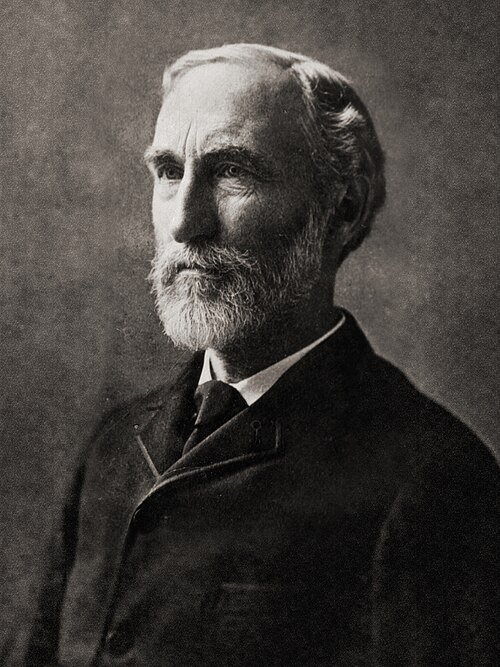
\includegraphics[width=\linewidth]{images/book3/gibbs.jpg}
\end{minipage}\hfill
\begin{minipage}[t]{0.76\linewidth}\vspace{0pt}
Josiah Willard Gibbs (1839--1903), profesor fisika matematika di Yale,
antara tahun 1876 dan 1878 menerbitkan \emph{On the Equilibrium of
Heterogeneous Substances}, sekitar tiga ratus halaman dalam terbitan
sebuah akademi kecil, tempat energi bebas, potensial kimia, dan aturan
fase dari bab-bab berikutnya semuanya muncul. Hanya sedikit kimiawan yang
membacanya sampai karya itu diterjemahkan pada tahun 1890-an. (Foto:
domain publik, Wikimedia Commons.)
\end{minipage}
\end{history}

\section{Energi Gibbs reaksi standar dan suhu}

\begin{definition}[Pendekatan Ellingham]\label{def:b2:reaction-free-energy:ellingham-approximation}
Yang disebut \emph{pendekatan Ellingham}\index{pendekatan Ellingham}
menganggap $\Delta_r H^\circ$ dan $\Delta_r S^\circ$ tidak bergantung pada
suhu dalam selang yang tidak memuat perubahan wujud. Maka
$\Delta_r G^\circ(T)
= \Delta_r H^\circ - T\Delta_r S^\circ$ merupakan
garis lurus terhadap $T$, dengan kemiringan $-\Delta_r S^\circ$.
\end{definition}

\begin{proposition}[Turunan terhadap suhu]\label{prop:b2:reaction-free-energy:gibbs-helmholtz}
\[
  \frac{\dd\Delta_r G^\circ}{\dd T} = -\Delta_r S^\circ, \qquad
  \frac{\dd}{\dd T}\!\left(\frac{\Delta_r G^\circ}{T}\right) =
  -\frac{\Delta_r H^\circ}{T^2}\ \ \text{(Gibbs--Helmholtz)}, \qquad
  \frac{\dd\Delta_r S^\circ}{\dd T} = \frac{\Delta_r C^\circ_p}{T}.
\]
Khususnya, \omterm{def:b2:reaction-free-energy:ellingham-approximation}{pendekatan Ellingham} berlaku jika $\Delta_r C^\circ_p$
kecil.
\end{proposition}

\begin{proof}
Dengan setiap spesies dalam keadaan standarnya, $G^\circ(T, \xi)$
memenuhi $(\partial
G^\circ/\partial T)_\xi = -S^\circ$
(\cref{prop:b2:reaction-free-energy:dG}). Menurut teorema Schwarz,
\[
  \frac{\dd\Delta_r G^\circ}{\dd T} = \partial_\xi\partial_T G^\circ =
  -\partial_\xi S^\circ = -\Delta_r S^\circ .
\] Kemudian $\frac{\dd}{\dd
T}(\Delta_r G^\circ/T) = \frac{-T\Delta_r S^\circ - \Delta_r G^\circ}{T^2} =
-\frac{\Delta_r H^\circ}{T^2}$. Akhirnya, $\dd S^\circ_m = C^\circ_{p,m}\,\dd
T/T$ untuk setiap spesies (\cref{prop:b2:reaction-free-energy:absolute-entropy}),
dan kombinasi yang sama memberikan hubungan terakhir. Jika
$\Delta_r C^\circ_p$ kecil, $\Delta_r H^\circ$ (Kirchhoff) dan
$\Delta_r S^\circ$ hampir tidak berubah.
\end{proof}

\begin{definition}[Suhu inversi]\label{def:b2:reaction-free-energy:inversion-temperature}
Jika $\Delta_r H^\circ$ dan $\Delta_r S^\circ$ bertanda sama, yang disebut
\emph{suhu inversi}\index{suhu inversi} reaksi itu adalah suhu tempat
$\Delta_r G^\circ$ berganti tanda; dalam \omterm{def:b2:reaction-free-energy:ellingham-approximation}{pendekatan Ellingham},
$T_i = \Delta_r H^\circ/\Delta_r S^\circ$.
\end{definition}

\begin{omfigure}
\begin{tikzpicture}
\begin{axis}[
  width=0.72\linewidth, height=5.6cm, xmin=0, xmax=1600, ymin=0, ymax=260,
  axis x line=bottom, axis y line=left, xlabel={$T$ (K)}, ylabel={\unit{kJ/mol}},
  tick label style={font=\small}, label style={font=\small}, clip=false]
\addplot[omThm, very thick] table[x=T, y=DrH] {figdata/out/bachelor-2-thermo-data-calcite.dat};
\addplot[omDef, very thick] table[x=T, y=TDrS] {figdata/out/bachelor-2-thermo-data-calcite.dat};
\node[omThm, anchor=south west, font=\small] at (axis cs:60,180) {$\Delta_r H^\circ = 178.3$};
\node[omDef, anchor=west, font=\small] at (axis cs:1600,257) {$T\Delta_r S^\circ$};
\draw[dotted] (axis cs:1110,0) -- (axis cs:1110,178.3);
\node[anchor=south west, font=\small] at (axis cs:1120,8) {$T_i = \qty{1110}{K}$};
\node[font=\scriptsize, align=center] at (axis cs:600,140) {$\Delta_r G^\circ > 0$:\\ kalsit stabil};
\node[font=\scriptsize, align=center] at (axis cs:1470,206) {$\Delta_r G^\circ < 0$};
\end{axis}
\end{tikzpicture}

{\small Suku entalpi dan suku entropi \ce{CaCO3(s) -> CaO(s) + CO2(g)}
dalam \omterm{def:b2:reaction-free-energy:ellingham-approximation}{pendekatan Ellingham}. Di bawah \omterm{def:b2:reaction-free-energy:inversion-temperature}{suhu inversi}, biaya entalpi menang
dan batu kapur stabil di bawah \qty{1}{bar} karbon dioksida; di atasnya,
suku entropi menang dan batu kapur terurai.}
% ledger: dfh:CaCO3_cr, dfh:CaO_cr, dfh:CO2, s0:CaCO3_cr, s0:CaO_cr, s0:CO2_g (computed in figdata/bachelor-2/thermo-data.py)
\end{omfigure}

\begin{omfigure}
\begin{tikzpicture}[font=\small]
  \draw[thick] (0,0) rectangle (8,4);
  \draw[thick] (4,0) -- (4,4) (0,2) -- (8,2);
  \node[above] at (2,4) {$\Delta_r H^\circ < 0$};
  \node[above] at (6,4) {$\Delta_r H^\circ > 0$};
  \node[left] at (0,3) {$\Delta_r S^\circ > 0$};
  \node[left] at (0,1) {$\Delta_r S^\circ < 0$};
  \node[align=center, omDef] at (2,3) {eksergonik\\ pada setiap $T$};
  \node[align=center, omProp] at (6,3) {eksergonik\\ di atas $T_i$};
  \node[align=center, omProp] at (2,1) {eksergonik\\ di bawah $T_i$};
  \node[align=center, omThm] at (6,1) {endergonik\\ pada setiap $T$};
\end{tikzpicture}

{\small Empat kasus $\Delta_r G^\circ = \Delta_r H^\circ - T\Delta_r
S^\circ$ (\omterm{def:b2:reaction-free-energy:ellingham-approximation}{pendekatan Ellingham}). Reaksi pembakaran berada di kotak kiri
atas; penguraian batu kapur dan kompres dingin di kanan atas; sintesis
amonia di kiri bawah.}
\end{omfigure}

\begin{method}[Energi Gibbs reaksi standar pada suhu $T$]\label{met:b2:reaction-free-energy:delta-g-standard}
\begin{enumerate}
  \item Dari tabel pada \qty{298.15}{K}, hitunglah $\Delta_r H^\circ$ dan
        $\Delta_r S^\circ$.
  \item Periksalah bahwa tidak ada spesies yang berubah wujud antara
        \qty{298}{K} dan $T$; jika ada, tambahkan transisinya (entalpi dan
        entropi) atau mulailah dari wujud yang baru.
  \item Dalam \omterm{def:b2:reaction-free-energy:ellingham-approximation}{pendekatan Ellingham}, $\Delta_r G^\circ(T) = \Delta_r H^\circ
        - T\Delta_r S^\circ$.
  \item Jika $\Delta_r C^\circ_p$ tidak kecil atau selangnya panjang,
        gunakan langsung $\Delta_f G^\circ(T)$ yang ditabelkan.
\end{enumerate}
\end{method}

\begin{example}[Dua uji pendekatan itu]\label{ex:b2:reaction-free-energy:tests}
Untuk batu kapur, $\Delta_r C^\circ_p = 42.80 + 37.13 - 81.88 =
\qty{-2.0}{J/(K.mol)}$: pendekatannya sangat baik, dan $\Delta_r
G^\circ = 178.3 - T \times 0.1606$ memberikan $T_i = \qty{1110}{K}$. Untuk
amonia, $\Delta_r G^\circ(700) \approx -91.9 + 700 \times 0.1981 =
\qty{+46.8}{kJ/mol}$, sedangkan tabel memberikan
$2\Delta_f G^\circ(\ce{NH3}, 700) =
\qty{+54.4}{kJ/mol}$: di sini
$\Delta_r C^\circ_p = \qty{-44}{J/(K.mol)}$ dan galatnya \qty{8}{kJ/mol},
faktor 4 pada tetapan kesetimbangan pada suhu itu.
% ledger: cp:CaO_cr.298, cp:CO2_g.298, cp:CaCO3_cr.298, janafG:NH3.700 (computed in figdata/bachelor-2/thermo-data.py)
\end{example}

\section{Latihan}

\begin{exercise}[$\star$]\label{exo:b2:reaction-free-energy:1}
Ramalkan tanda $\Delta_r S^\circ$ untuk: (a) \ce{2H2(g) + O2(g) -> 2H2O(l)};
(b) \ce{CaCO3(s) -> CaO(s) + CO2(g)}; (c) \ce{N2O4(g) -> 2NO2(g)};
(d) \ce{Ag+(aq) + Cl-(aq) -> AgCl(s)}; (e) \ce{H2O(s) -> H2O(l)};
(f) \ce{H2(g) + Cl2(g) -> 2HCl(g)}.
\end{exercise}

\begin{exercise}[$\star$]\label{exo:b2:reaction-free-energy:2}
Hitunglah $\Delta_r S^\circ$ dan $\Delta_r G^\circ$ pada \qty{298.15}{K}
untuk sintesis amonia, \ce{N2(g) + 3H2(g) -> 2NH3(g)}, dengan
$\Delta_r
H^\circ = \qty{-91.9}{kJ/mol}$ dan entropi dalam bab ini.
Apakah reaksi itu \omterm{def:b2:reaction-free-energy:exergonic}{eksergonik}?
\end{exercise}

\begin{exercise}[$\star$]\label{exo:b2:reaction-free-energy:3}
Hitunglah $\Delta_r G^\circ(\qty{298.15}{K})$ untuk \ce{H2(g) + 1/2O2(g) ->
H2O(l)} dari $\Delta_f H^\circ(\ce{H2O}, \text{l}) = \qty{-285.83}{kJ/mol}$
dan entropi standar \ce{H2(g)} 130.68, \ce{O2(g)} 205.15, \ce{H2O(l)}
\qty{69.95}{J/(K.mol)}. Mengapa nilai ini merupakan \omterm{def:b2:reaction-free-energy:gibbs-energy}{energi Gibbs}
pembentukan standar air cair?
% ledger: dfh:H2O-l, s0:H2_g, s0:O2_g, s0:H2O_l
\end{exercise}

\begin{exercise}[$\star$]\label{exo:b2:reaction-free-energy:4}
Gunakan gambar entropi seng untuk membaca \omterm{def:b2:reaction-free-energy:standard-entropy}{entropi molar standarnya} pada
\qty{298}{K} dan pada \qty{1000}{K}, serta lonjakannya pada titik lebur
dan titik didih. Simpulkan entalpi peleburan dan entalpi penguapannya.
\end{exercise}

\begin{exercise}[$\star\star$]\label{exo:b2:reaction-free-energy:5}
Untuk \ce{H2O(l) -> H2O(g)} pada \qty{298.15}{K}, hitunglah
$\Delta_r H^\circ$, $\Delta_r S^\circ$, dan $\Delta_r G^\circ$ dari tabel
dalam bab ini. Jelaskan mengapa $\Delta_r S^\circ \neq \Delta_r H^\circ/T$
pada \qty{298}{K}, apa arti $\Delta_r G^\circ$ yang positif, lalu
perkirakan dengan \omterm{def:b2:reaction-free-energy:ellingham-approximation}{pendekatan Ellingham} suhu pada saat air cair dan uapnya
pada \qty{1}{bar} berada dalam kesetimbangan. Bandingkan dengan titik
didihnya.
\end{exercise}

\begin{exercise}[$\star\star$]\label{exo:b2:reaction-free-energy:6}
Untuk \ce{N2O4(g) -> 2NO2(g)}, $\Delta_r H^\circ = \qty{57.1}{kJ/mol}$ dan
$\Delta_r S^\circ = \qty{175.7}{J/(K.mol)}$. Hitunglah \omterm{def:b2:reaction-free-energy:inversion-temperature}{suhu inversinya},
lalu jelaskan mengapa tabung tertutup berisi gas cokelat \ce{NO2} menjadi
pucat ketika didinginkan dalam es.
\end{exercise}

\begin{exercise}[$\star\star$]\label{exo:b2:reaction-free-energy:7}
Sebuah reaksi mempunyai $\Delta_r G^\circ = \qty{-12.0}{kJ/mol}$ pada
\qty{300}{K} dan $\qty{-4.0}{kJ/mol}$ pada \qty{400}{K}. Dalam \omterm{def:b2:reaction-free-energy:ellingham-approximation}{pendekatan
Ellingham}, tentukan $\Delta_r H^\circ$ dan $\Delta_r S^\circ$, lalu
periksalah hubungan Gibbs--Helmholtz.
\end{exercise}

\begin{exercise}[$\star\star$]\label{exo:b2:reaction-free-energy:8}
Hitunglah $\Delta_r G^\circ$ pembentukan metana, \ce{C(s) + 2H2(g) ->
CH4(g)}, pada \qty{298.15}{K}, dari $\Delta_f H^\circ = \qty{-74.87}{kJ/mol}$
dan entropi \ce{C} (grafit) 5.74, \ce{H2} 130.68, \ce{CH4}
\qty{186.25}{J/(K.mol)}. Di atas suhu berapakah metana menjadi tidak
stabil terhadap unsur-unsurnya pada tekanan standar?
% ledger: dfh:CH4_g, s0:C_gr, s0:H2_g, s0:CH4_g
\end{exercise}

\begin{exercise}[$\star\star$]\label{exo:b2:reaction-free-energy:9}
Sebuah haloalkana bereaksi dengan basa melalui substitusi atau
eliminasi. Tuliskan kedua reaksi untuk 2-bromopropana dan hidroksida.
Dengan $\Delta_r
H^\circ(\text{eliminasi}) - \Delta_r H^\circ(\text{substitusi}) =
\qty{+40}{kJ/mol}$ dan $\Delta_r S^\circ(\text{eliminasi}) - \Delta_r
S^\circ(\text{substitusi}) = \qty{+90}{J/(K.mol)}$ (orde besaran),
tentukan di atas suhu berapa eliminasi menjadi reaksi yang lebih
\omterm{def:b2:reaction-free-energy:exergonic}{eksergonik} di antara keduanya, lalu jelaskan peran jumlah molekul.
\end{exercise}

\begin{exercise}[$\star\star\star$]\label{exo:b2:reaction-free-energy:10}
Karbon monoksida kristal tidak mencapai entropi nol pada \qty{0}{K}:
setiap molekul dapat terletak sebagai CO atau OC hampir secara acak,
karena kedua orientasi itu mempunyai energi yang hampir sama. Dengan
menerima rumus Boltzmann $S = k_B\ln W$, dengan $W$ jumlah susunan
(dihitung dalam jilid Tahun 3), hitunglah entropi molar sisanya. Mengapa
hukum ketiga tidak berlaku untuk kristal ini?
\end{exercise}

\begin{exercise}[$\star\star\star$]\label{exo:b2:reaction-free-energy:11}
Tunjukkan bahwa jika $\Delta_r C^\circ_p$ adalah tetapan $c$,
$\Delta_r S^\circ(T) = \Delta_r S^\circ(T_0) + c\ln(T/T_0)$ dan
$\Delta_r G^\circ(T) = \Delta_r H^\circ(T_0) - T\Delta_r S^\circ(T_0) +
c\,[T - T_0 - T\ln(T/T_0)]$. Terapkan pada batu kapur ($c =
\qty{-2.0}{J/(K.mol)}$) pada \qty{1100}{K}, lalu ukurlah galat
\omterm{def:b2:reaction-free-energy:ellingham-approximation}{pendekatan Ellingham}.
\end{exercise}

\begin{exercise}[$\star\star\star$]\label{exo:b2:reaction-free-energy:12}
Titanium dibuat dari oksidanya, rutil, melalui kloridanya. (a) Hitunglah
$\Delta_r H^\circ$ dan $\Delta_r S^\circ$ pada \qty{298}{K} untuk
\ce{TiO2(s) +
2Cl2(g) -> TiCl4(g) + O2(g)}, dengan \ce{TiO2} ($-944.0$
\unit{kJ/mol}, \qty{50.62}{J/(K.mol)}) dan \ce{TiCl4(g)} ($-763.2$, 353.2),
serta $\Delta_r G^\circ$-nya pada \qty{1000}{K} dalam \omterm{def:b2:reaction-free-energy:ellingham-approximation}{pendekatan
Ellingham}. (b) Karbon ditambahkan: \ce{C(s) + O2(g) -> CO2(g)},
$\Delta_r H^\circ =
\qty{-393.5}{kJ/mol}$, $\Delta_r S^\circ = \qty{+2.9}{J/(K.mol)}$. Hitunglah $\Delta_r G^\circ(\qty{1000}{K})$ untuk
jumlah kedua reaksi itu, lalu jelaskan bagaimana reaksi kedua mendorong
reaksi pertama.
% ledger: dfh:TiO2_cr, s0:TiO2_cr, dfh:TiCl4_g, s0:TiCl4_g, s0:Cl2_g, s0:O2_g, s0:C_gr, s0:CO2_g
\end{exercise}

\section{Soal: Tungku Kapur}

\begin{problem}[{Soal akhir pekan --- entropi dan entalpi sebuah
penguraian, energi Gibbs-nya terhadap suhu, kriteria evolusi di dalam
tungku, serta energi dan karbon dioksida untuk satu ton kapur tohor}]
\label{pb:b2:reaction-free-energy:1}
Kapur tohor, \ce{CaO}, dibuat dengan memanaskan batu kapur, \ce{CaCO3},
di dalam tungku. Data pada \qty{298.15}{K}: $\Delta_f H^\circ$
(\unit{kJ/mol}) \ce{CaCO3(s)} $-1206.92$, \ce{CaO(s)} $-635.09$,
\ce{CO2(g)} $-393.51$; $S^\circ_m$ (\unit{J/(K.mol)}) 92.9, 39.75, 213.79;
$C^\circ_{p,m}$ (\unit{J/(K.mol)}) 81.88, 42.80, 37.13. Massa molar:
\ce{CaO} \qty{56.08}{g/mol}, \ce{CO2} \qty{44.01}{g/mol}, \ce{CH4}
\qty{16.04}{g/mol}; pembakaran metana, dengan air berupa uap,
$\Delta_r H^\circ = \qty{-802.3}{kJ/mol}$.
% ledger: dfh:CaCO3_cr, dfh:CaO_cr, dfh:CO2, s0:CaCO3_cr, s0:CaO_cr, s0:CO2_g, cp:CaCO3_cr.298, cp:CaO_cr.298, cp:CO2_g.298

\medskip
\noindent\textbf{Bagian I --- Pada suhu kamar.}
\begin{enumerate}
  \item Tuliskan reaksi penguraian batu kapur.
  \item Hitunglah $\Delta_r H^\circ(\qty{298}{K})$. Apakah reaksi itu
        \omterm{def:b2:reaction-enthalpy:exothermic}{eksoterm}?
  \item Hitunglah $\Delta_r S^\circ(\qty{298}{K})$ dan jelaskan tandanya.
  \item Hitunglah $\Delta_r G^\circ(\qty{298}{K})$.
  \item Apakah batu kapur stabil pada suhu kamar di bawah \qty{1}{bar}
        karbon dioksida? Mengapa tebing-tebing kapur dapat bertahan?
  \item Hitunglah $\Delta_r C^\circ_p$, lalu nyatakan apa akibatnya bagi
        kebergantungan $\Delta_r H^\circ$ dan $\Delta_r S^\circ$ pada
        suhu.
\end{enumerate}

\medskip
\noindent\textbf{Bagian II --- Pemanasan.}
\begin{enumerate}[resume]
  \item Tuliskan $\Delta_r G^\circ(T)$ dalam \omterm{def:b2:reaction-free-energy:ellingham-approximation}{pendekatan Ellingham}.
  \item Hitunglah nilainya pada \qty{1000}{K} dan pada \qty{1300}{K}.
  \item Hitunglah \omterm{def:b2:reaction-free-energy:inversion-temperature}{suhu inversi} $T_i$.
  \item Periksalah hubungan Gibbs--Helmholtz pada ungkapan ini.
  \item Perkirakan, dengan rumus pada \cref{exo:b2:reaction-free-energy:11},
        perubahan $\Delta_r G^\circ$ pada $T_i$ yang disebabkan oleh
        $\Delta_r C^\circ_p$, serta pergeseran $T_i$ yang ditimbulkannya.
\end{enumerate}

\medskip
\noindent\textbf{Bagian III --- Tungku.}
Dalam bagian ini karbon dioksida di atas padatan berada pada \qty{1}{bar},
sehingga $\Delta_r G = \Delta_r G^\circ$.
\begin{enumerate}[resume]
  \item Apa yang dinyatakan kriteria evolusi pada \qty{1000}{K}? Dan pada
        \qty{1300}{K}?
  \item Apa yang terjadi pada campuran kapur tohor dan karbon dioksida
        pada \qty{1}{bar} yang didinginkan di bawah $T_i$?
  \item Berapa entropi yang tercipta per mol batu kapur yang terurai pada
        \qty{1300}{K}?
  \item Tungku disapu oleh gas pembakaran, yang lebih miskin karbon
        dioksida. Tebaklah, sebelum bab berikutnya, apakah hal ini
        membantu penguraian.
\end{enumerate}

\medskip
\noindent\textbf{Bagian IV --- Satu ton kapur tohor.}
\begin{enumerate}[resume]
  \item Hitunglah jumlah kapur tohor dalam satu ton.
  \item Hitunglah kalor yang diserap oleh reaksi per ton kapur tohor
        (anggaplah $\Delta_r H^\circ$ tetap).
  \item Hitunglah massa karbon dioksida yang dilepaskan oleh batu kapur
        per ton kapur tohor.
  \item Kalor itu berasal dari pembakaran metana dengan efisiensi berguna
        50\,\%. Hitunglah massa metana yang dibakar per ton kapur tohor.
  \item Hitunglah karbon dioksida dari metana ini.
  \item Hitunglah total karbon dioksida per ton kapur tohor, serta bagian
        yang berasal dari batu kapur itu sendiri.
  \item Mengapa bahan bakar yang lebih bersih hanya dapat mengurangi
        sebagian dari emisi ini?
  \item Nyatakan suhu yang di atasnya batu kapur terurai di bawah
        \qty{1}{bar} karbon dioksida.
\end{enumerate}
\end{problem}
